\documentclass[12pt, a4paper] {ncc}
\usepackage[utf8] {inputenc}
\usepackage[T2A]{fontenc}
\usepackage[english, russian] {babel}
\usepackage[usenames,dvipsnames]{xcolor}
\usepackage{listings,a4wide,longtable,amsmath,amsfonts,graphicx}
\usepackage{indentfirst}
\usepackage{bytefield}
\usepackage{multirow}
\usepackage{float}
\usepackage{caption}
\usepackage{subcaption}
\captionsetup{compatibility=false}
\usepackage{tabularx}
\usepackage{pdfpages}

\usepackage[left=2cm,right=2cm,top=2cm,bottom=2cm,bindingoffset=0cm]{geometry}

\begin{document}
\setcounter{figure}{0}
\frenchspacing
\pagestyle{empty}
\begin{center}
                            Университет ИТМО    \\
					Мегафакультет компьютерных технологий и управления \\ 
					Факультет программной инженерии и компьютерной техники \\
                        Кафедра вычислительной техники

\vspace{\stretch{2}}
                Системы ввода/вывода и периферийные устройства
\end{center}
\vspace{\stretch{2}}
\begin{center}

                Лабораторная работа №3\\
			{\it «Разработка и прототипирование контроллеров 
                ввода/вывода с использованием языка Verilog HDL на ПЛИС»}

					Вариант 8
\end{center}
\vspace{\stretch{3}}
\begin{flushright}
                                    Студенты:\\
                                    {\it Куклина М.Д.}\\
                                    {\it Кириллова А.А.}\\
                                    Преподаватель: \\
                                    {\it Быковский С.В.}
\end{flushright}
\vspace{\stretch{4}}
\begin{center}
                             Санкт-Петербург, 2017
\end{center}
\newpage

%\tableofcontent

\section{Задание}

Программное обеспечение soft-процессора Microblaze должно выполнять 
функции программного обеспечения из Лабораторной работы №1 и №2. 
 
Программное обеспечение Microblaze должно распознавать последовательность 
011 (двоичное число, 3 бита) и определять длительность каждого символа с 
помощью блока AXI Timer. Длительность символа в нс необходимо выводить на 
дискретные порты ввода/ вывода блока AXI GPIO. По факту распознания 
последовательности на дискретные порты блока AXI GPIO однократно выводится 
значение 0xFFFF. 
 
Блок Output Compare должен быть настроен на генерацию последовательности 
011 (двоичное число, 3 бита) с заданной длительностью каждого символа. 
Длительность каждого символа передается по последовательному каналу и 
принимается с помощью блока AXI Uartlite. 
 
В аппаратном обеспечении выход outs блока Output Compare подается на вход 
capturetrig0  блока AXI Timer. 

\section{Структурная схема разработанной системы}
	См. приложение.

\section{Блок-схема организации ПО процессора}

	Совпадает с организацией ПО процессора в прошлой лабораторной работы, исключая
	дополнительную настройку блока {\it OutputCompare}, которая в блок-схеме не
	нуждается.

\section{Временные диаграммы}

	Временные диаграммы для символов размера 300.

	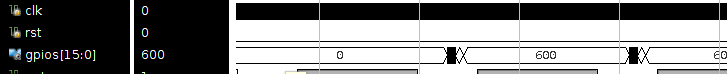
\includegraphics[scale=0.5]{./600_close.png}

	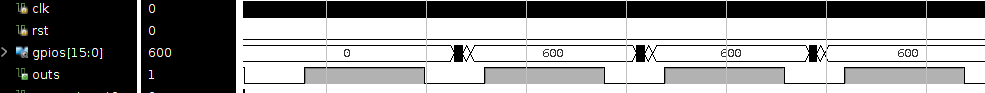
\includegraphics[scale=0.5]{./600_not_too_close.png}
	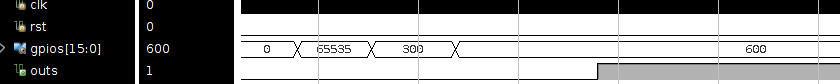
\includegraphics[scale=0.5]{./600_too_close.png}


\section{Выводы}

В ходе лабораторной работы был разработан контроллер ввода/вывода и программное
обеспечение для него.

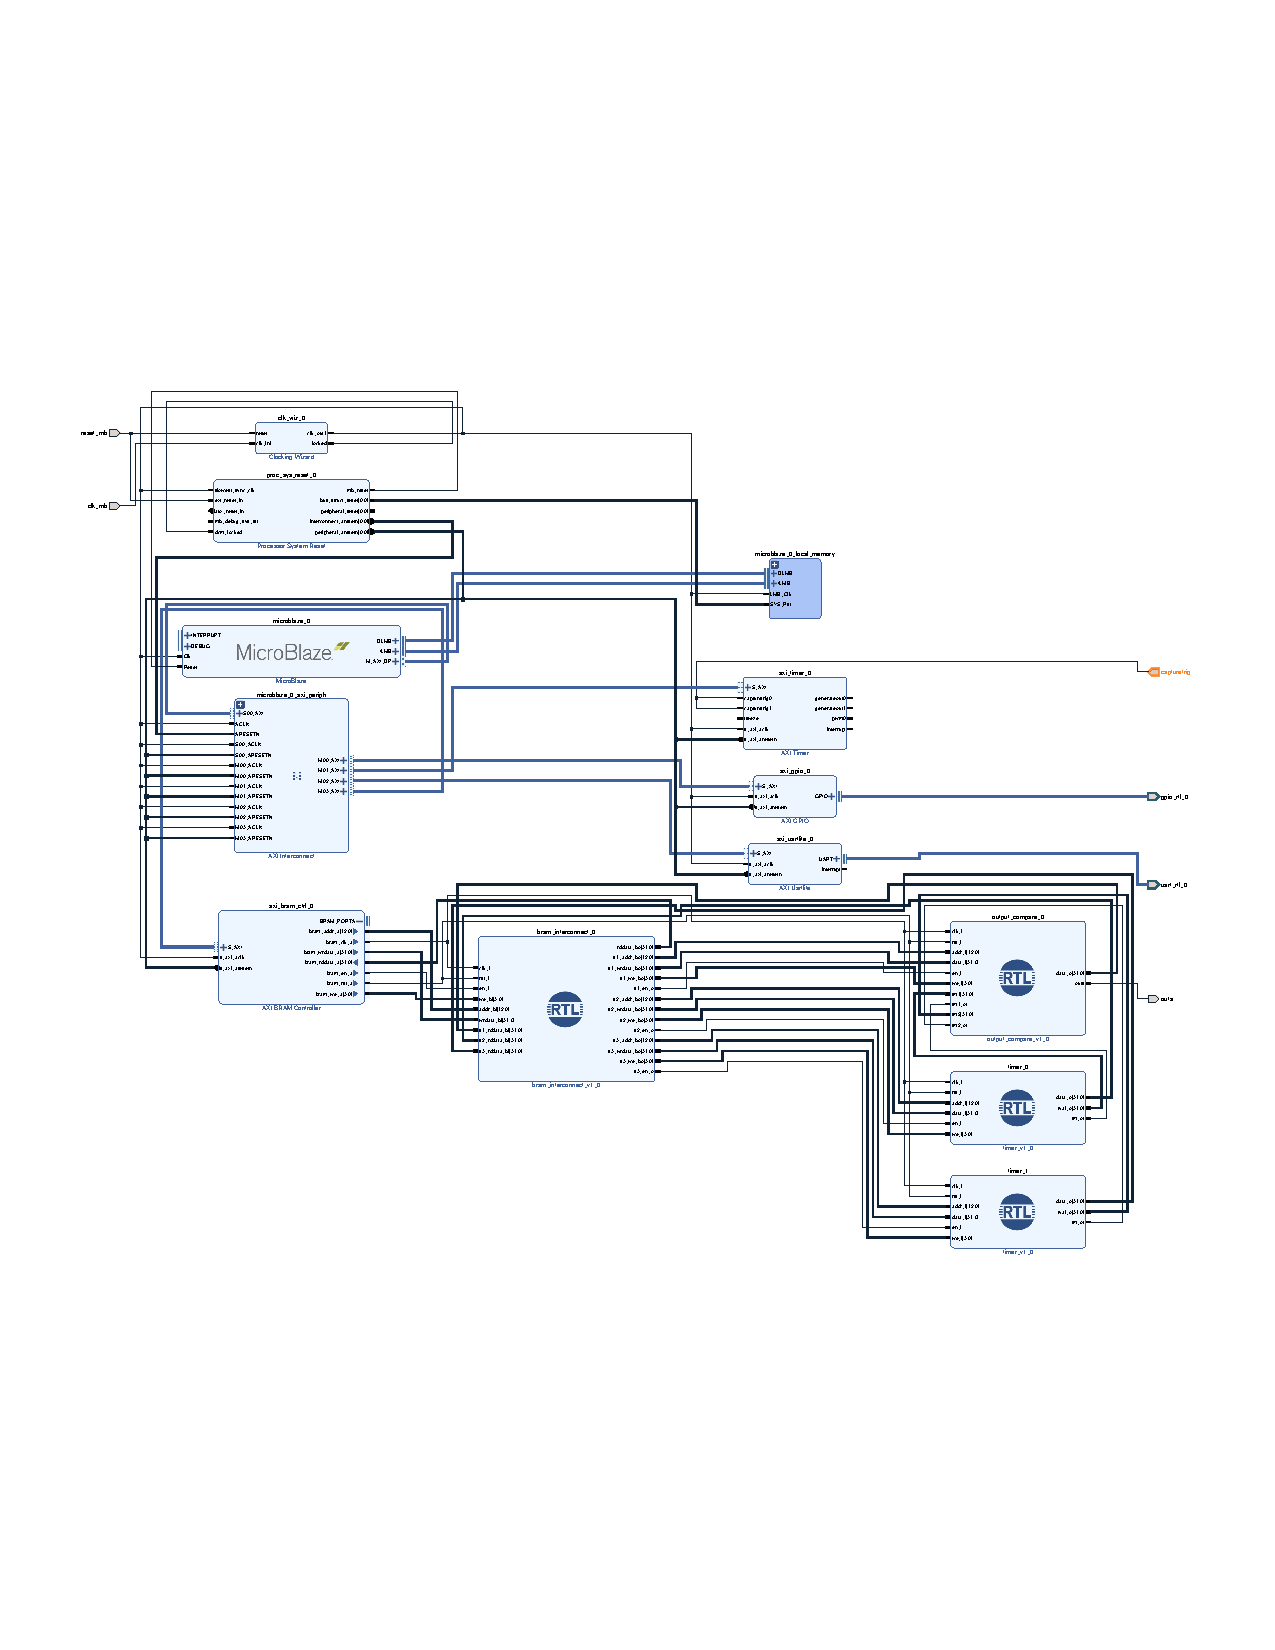
\includepdf[pages={1}]{uc_system.pdf}
 
\end{document}
